\documentclass[10pt]{article}

\usepackage[table,svgnames]{xcolor}
\usepackage{color}
\usepackage{hyperref}
\usepackage{graphicx}
\usepackage{multirow}
\usepackage{multicol}
\usepackage{tikz}
\usepackage{pgfplots}
\usetikzlibrary{shapes,arrows,matrix}
\usepackage{fancyhdr}
\usepackage{epigraph}
\usepackage{listings}
\usepackage{lastpage}
\usepackage{smartdiagram}
\usepackage{caption}
\usepackage{sectsty}
\usepackage{mathtools}

\definecolor{PCFTorange}{RGB}{145,34,5}
\definecolor{PCFTorangedark}{RGB}{79,26,12}
\definecolor{PCFTorangelight}{RGB}{255,96,62}

\allsectionsfont{\color{PCFTorangedark}}

\lstset{
  basicstyle=\small\ttfamily,
  keywordstyle=\color{blue},
  showstringspaces=false,
  frame=shadowbox,
  rulesepcolor=\color{PCFTorangedark},
  backgroundcolor=\color{lightgray},
  numberstyle=\small\color{gray},
  tabsize=2,
  numbers=left,
  breaklines=true,
  postbreak=\mbox{\textcolor{red}{$\hookrightarrow$}\space},
}

\lstdefinelanguage{lua}{
  morekeywords={
    function, local, return, end
 },
 keywordstyle=[2]{\textbf},
 morecomment=[l]{--},
 morestring=[b]{'},
 tabsize=4}

\title{\color{PCFTorangedark} \textbf{Pcraft Handbook\\ a companion to Pcraft}}
\author{Sebastien Tricaud $<$sebastien.tricaud@devo.com$>$\\
  Lead Developer of Pcraft\\
  \url{http://www.github.com/devoinc/pcraft}
}



%% Footer
\renewcommand{\footrulewidth}{0.4pt}
\cfoot{This is Pcraft Handbook. The Opensource crafting document released under MIT License.}



\begin{document}
\maketitle

\begin{center}

\includegraphics[width=4cm]{pcraft-logo.png}
\end{center}

\vspace{0.5in}

\begin{abstract}

\renewcommand{\epigraphflush}{center}
\begin{epigraphs}
\centering
\setlength{\epigraphwidth}{1.6\textwidth}
\qitem{Those are my principles, and if you don't like them... well, I have others.}{---\textsc{Groucho Marx}}
\end{epigraphs}

\vspace{1in}

Pcraft originally meant  ``Packet Crafter'', but now does much more! It is available from \url{http://www.github.com/devoinc/pcraft}. Pcraft will help you archive three things:
\begin{enumerate}
\item Define Attack Scenarios (using the AMI language)
\item Create a Packet Capture (pcap) from an Attack Scenario
\item Write Logs for Simulated Devices
\end{enumerate}

\end{abstract}

{
\begin{figure}
\begin{center}
\caption{\textbf{Document Status}}
{\rowcolors{2}{PCFTorange}{PCFTorangelight}
\begin{tabular}{|c|l|l|}
\hline
\textbf{Date} & \textbf{Author} & \textbf{Description} \\
\hline
\today & Sebastien Tricaud & First version \\
\hline
\end{tabular}
}
\end{center}
\end{figure}
}

\newpage

\tableofcontents

\newpage

\section{Introduction}

This Handbook will walk the reader through all the capability Pcraft gives. 

\subsection{Pcraft overview}

Pcraft generates consistent logs across a variety of devices/applications. To achieve that, it uses a language called AMI, which sole purpose
is to \textbf{describe} what is expected. This is called a scenario as it contains the script that will drive Pcraft through the various steps it
requires to complete the job.

The advantage of this scenario is its reading simplicity.

Once the scenario is written, Pcraft needs to create a database that can be either in Pcap or in Avro. We will get into details of those two ways later in the handbook. From the database output, it is read to create logs for the supported devices/applications.

An overview of the various steps using the Pcap for the database can be summarized in the following graph:
\begin{center}
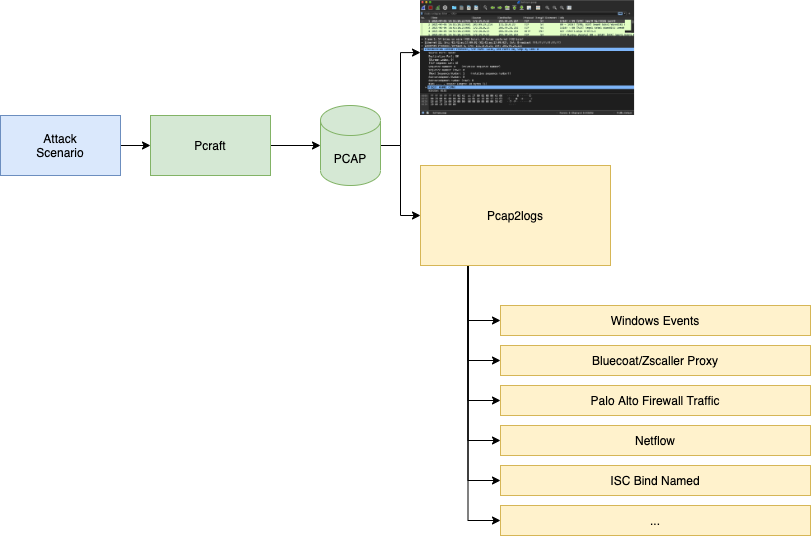
\includegraphics[width=\textwidth]{architecture.png}
\end{center}


\subsection{Creating DNS bind logs}

Writing a DNS connection requires using the plugin \textbf{DNSConnection} inside an action block. Each action done is wrapped into an action block. There can be as many action block as required. Also the \textbf{av 1} in the header is mandatory, it helps to version the actual language specification so the AMI language can evolve in the future while preserving backward compatibility. \textbf{av} is short for \textbf{ami\_version} which can also be used instead.

\begin{lstlisting}[caption={AMI file to create DNS bind logs},captionpos=b]
  av 1

  action dns {
    $domain = "example.com"
    exec DNSConnection
  }  
\end{lstlisting}

This action generates three files:

\begin{center}
\begin{tabular}{|l|l|}
  \hline
  \textbf{File Name} & \textbf{Description} \\
  \hline
 bind\_query.log & DNS Bind query log\\
  \hline
 netflow\_v9.log & Netflow v9 log\\
  \hline
 paloalto\_firewall.log & Palo Alto firewall log\\
  \hline
\end{tabular}
\end{center}

\vspace{1em}

The file \textit{bind\_query.log} contains the following:
\begin{lstlisting}[caption={bind\_query.log output},captionpos=b]
  0,14-Jul-2021 17:42:02.000000 queries: info: client 192.168.191.70#31928: query: example.com A IN + (1.1.1.1)  
\end{lstlisting}

Which is exactly what the \textbf{Bind Named daemon} would have written. In this case however, the source IP making the request, as well as the resolver have not been defined in the AMI scenario, which made Pcraft choosing for default values.

\section{Pcraft Tools}

Pcraft is actually the project name for several tools. This section covers what they are so you can decide what is best.

\subsection{The Packet Capture world}
The original project was simply a pcap writer to then extract logs for it. If we take the DNS query AMI example seen in the introduction section, it is contained in a file called \textit{dns.ami}; To generate a pcap from this file, the \textbf{pcrafter} program can be run:

\begin{lstlisting}[caption={Writing a pcap},captionpos=b]
$ /pcrafter dns.ami dns.pcap
Opening Script File dns.ami
Scenariofile: [dns.ami]
All plugins loaded!
Final Sleep Cursor: 0 seconds; 0 hours; 0 days
0 writing errors
\end{lstlisting}

We now have \textit{dns.pcap} which contains the request and reply to it, we can use any tool that can read a pcap, as it is a standardized format. For example with tshark:
\begin{lstlisting}[caption={Reading dns.pcap using tshark},captionpos=b]
$ tshark -r dns.pcap
    1   0.000000 192.168.133.32 ? 1.1.1.1      DNS 71 Standard query 0x0000 A example.com
    2   0.000000      1.1.1.1 ? 192.168.133.32 DNS 98 Standard query response 0x0000 A example.com A 10.140.81.215    
\end{lstlisting}

The next tool we want to use is \textbf{pcap2logs} which will write logs from simulated devices and application using this pcap as input. Note pcap2logs works with \textbf{any pcap}, including those which have not been generated using \textbf{pcrafter}. Here is how \textbf{pcap2logs} will generate logs:
\begin{lstlisting}[caption={Generating logs from a pcap},captionpos=b]
$ ./pcap2log.py dns.pcap dns
Loaded 21 plugins
{'http': ['bluecoat-proxysg-main', 'zscaler-access'], 'ntp': ['corelight-ntp'], 'no-active-layer': ['fidelis', 'hbss-agent', 'hbss-audit', 'hbss-epo', 'hbss-intrusion', 'mcafee-edr', 'mcafee-emailgateway', 'mswin-o365', 'mswin-powershell', 'mswin-security', 'mswin-sysmon', 'paloalto-threat', 'tanium'], 'dns': ['named'], 'ip': ['netflow', 'paloalto-firewall'], 'snmp': ['snmptrapd'], 'syslog': ['syslog']}
Layers that did not match a plugin: 4
Writer process done, now rewriting from config

$ ls dns/
bind_query.log	netflow_v9.log	paloalto_firewall.log  
\end{lstlisting}

To use \textbf{pcap2logs} the first parameter is the \textbf{pcap file} and the second the \textbf{output directory} where those logs must be written.

\subsection{The Avro database}

The pcap file is convenient, however limited by its writing speed simply because a pcap must be crafted with some extra data and consistency across each frame. While this speed does not matter to write a large amount of devices interracting with each other, Pcraft was designed to simulate real infrastructure with hundred of thousand devices. Hence Pcap will not be suitable for such a scale at this time.

The Avro database is simply the output of the data run from the AMI scenario file, to be used later to write logs. In order to write an Avro database and not a pcap, another tool must be used: \textbf{ccraft}.

\begin{lstlisting}[caption={Creating an Avro database},captionpos=b]
  $ ./ccraft/ccraft dns.ami dns.db
  Start Time: None
\end{lstlisting}

Notice the speed at which this is written. It is much faster than \textbf{pcrafter}.

Now the database is generated, it must be used to create logs from it. The tool used is called \textbf{db2logs}, as it translates this database into the logs using the same plugins as before.

\begin{lstlisting}[caption={Genering logs from an Avro database},captionpos=b]
./db2logs.py dns.db dns -f
Loaded 21 plugins
{'http': ['bluecoat-proxysg-main', 'zscaler-access'], 'ntp': ['corelight-ntp'], 'no-active-layer': ['fidelis', 'hbss-agent', 'hbss-audit', 'hbss-epo', 'hbss-intrusion', 'mcafee-edr', 'mcafee-emailgateway', 'mswin-o365', 'mswin-powershell', 'mswin-security', 'mswin-sysmon', 'paloalto-threat', 'tanium'], 'dns': ['named'], 'ip': ['netflow', 'paloalto-firewall'], 'snmp': ['snmptrapd'], 'syslog': ['syslog']}
\end{lstlisting}

\subsection{List of Pcraft tools}

  \hspace*{-1cm}\begin{tabular}{|c|l|l|}
    \hline
    \textbf{Tool Name} & \textbf{Description} & \textbf{Example use} \\
    \hline
    \textbf{pcrafter} & Generate a pcap from an AMI scenario & ./pcrafter dns.ami dns.pcap \\
    \hline
    \textbf{ccraft} & Generate an Avro database from an AMI scenario & ./ccraft/ccraft dns.ami dns.db \\
    \hline
    \textbf{pcap2logs} & Generate logs from a pcap & ./pcap2logs.py dns.pcap dns -f \\
    \hline
    \textbf{db2logs} & Generate logs from an Avro database & ./db2logs.py dns.db dns -f \\
    \hline
  \end{tabular}

\begin{center}
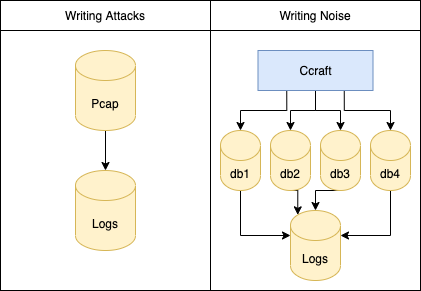
\includegraphics[width=\textwidth]{noise.png}
\end{center}

\section{Ami}

Ami is the language which powers Pcraft to generate data correctly. It offers a way to describe actions, repeat loops, and how long does one sleep until the next action. The reason for Ami to have been designed was looking at the requirements of what generating those data required. From running actions both in sequence and parallel, tied to a time sequence with variables that can be defined in either a given action, or from a called action execution.

To understand how Ami works, it is best to start with the famous "Hello, World!" example:
\begin{lstlisting}[caption={Hello world in Ami},captionpos=b]
  av 1

  action hello {
    exec Void
  }
\end{lstlisting}

Ami runs action, there must be at least one action block to execute something. In this case, \textbf{line 4} of the hello world example, we execute nothing (\textbf{Void}), which actually just dumps to the standard output the variables defined at this stage.

\textbf{Line 3} is the declaration of the action block, which takes a name that you want.

On \textbf{line 1}, this is a required header which defines the Ami Version, which must be 1 for now, but will evolve in the future to include more features and keep backward compatibility.

We can run this example using the \textbf{pcrafter} tool like this:
\begin{lstlisting}[caption={Running Hello world},captionpos=b]
./pcrafter hello.ami hello.pcap
Opening Script File hello.ami
Scenariofile: [hello.ami]
All plugins loaded!
{'__amifile__': 'hello.ami'}
Final Sleep Cursor: 0 seconds; 0 hours; 0 days
0 writing errors
\end{lstlisting}

As you can see there is a defined variable, called \textbf{\_\_amifile\_\_} which is an internal variable displaying the actual file name being parsed.

\subsection{Header keywords}

It is mendatory to start the Ami scenario using the \textbf{ami\_version} or \textbf{av} keyword, the others are optional but can strengthen the quality of the scenario, such as:

\begin{itemize}
\item \textbf{reference}: To set a reference string towards information used to build that scenario. We can add as many as necessary
\item \textbf{revision}: An integer to manually increment when work has been done on the file
\item \textbf{author}: To reference the file Author
\item \textbf{description}: A description about the scenario
\item \textbf{shortdesc}: A short description about the scenario
\item \textbf{tag}: A tag you may want to apply (similar to revision, there can be as many tags as needed
\item \textbf{start\_time}: To force a time start (in epoch)
\end{itemize}

\subsection{Variables}

In Ami, a variable is by default globally defined and accessible by the following actions. Which allows any execution plugin to create new ones to be used later. This is because any action can consume a previously defined variable to work. A Variable is declared with a \textbf{word} prepended with the \textbf{\$} dollar sign, such as:
\begin{equation}
  \boxed{\$hello = "world"}
\end{equation}

would set the string "world" to the \textbf{hello} variable.

If we take the previous example but adding this variable, we can see it printed now:
\begin{lstlisting}[caption={Hello world with a variable},captionpos=b]
  av 1

  action hello {
    $hello = "world"
    exec Void
  }
\end{lstlisting}

\begin{lstlisting}[caption={Running our example},captionpos=b]
$ ./pcrafter hello.ami hello.pcap
Opening Script File hello.ami
Scenariofile: [hello.ami]
All plugins loaded!
{'__amifile__': 'hello.ami', 'hello': 'world'}
Final Sleep Cursor: 0 seconds; 0 hours; 0 days
0 writing errors
\end{lstlisting}

We can see here the \textbf{world} string set to the \textbf{hello} variable.

If we run two consecutives actions, the \textbf{hello} variable would still be visible by the other block:
\begin{lstlisting}[caption={Hello world with a variable  and two action blocks},captionpos=b]
  av 1

  action hello {
    $hello = "world"
    exec Void
  }

  action second {
    exec Void
  }
\end{lstlisting}

\begin{lstlisting}[caption={Printing variables for each action},captionpos=b]
All plugins loaded!
{'__amifile__': 'hello.ami', 'hello': 'world'}
{'__amifile__': 'hello.ami', 'hello': 'world'}
Final Sleep Cursor: 0 seconds; 0 hours; 0 days
\end{lstlisting}

\textbf{Line 3} prints the variables for the action block \textbf{hello} and \textbf{line 4}  prints them for the block \textbf{second}. They both see the \textbf{hello} variable.

To stop a variable from being carried to the next action block, one can use the keyword \textbf{delete}, such as:
\begin{lstlisting}[caption={Deleting our variable},captionpos=b]
  av 1

  action hello {
    $hello = "world"
    exec Void
  }

  delete $hello
  
  action second {
    exec Void
  }
\end{lstlisting}

\subsection{Functions}

A Function can define the value to be set for a variable. The actual functions have been designed to help generating data faster, we can add as many as we see fit.

\subsubsection{Usage}
Let us start with an example, where we assign to a variable the base64 encoding of "Hello, world!":
\begin{lstlisting}[caption={Encoding a string},captionpos=b]
  av 1

  action hello {
    $mystr = base64.encode("Hello, world!")
    exec Void
  }
\end{lstlisting}

\begin{lstlisting}[caption={Seeing our encoded string},captionpos=b]
$ ./pcrafter hello.ami hello.pcap
Opening Script File hello.ami
Scenariofile: [hello.ami]
All plugins loaded!
{'__amifile__': 'hello.ami', 'mystr': 'SGVsbG8sIHdvcmxkIQ=='}
Final Sleep Cursor: 0 seconds; 0 hours; 0 days
0 writing errors
\end{lstlisting}

Functions can be recusively called, for example, if we want to get a random string of 10 characters, we can use the function \textbf{random.string(10)}, and to encode in base64 this string, we can write:
\begin{equation}
  \boxed{base64.encode(random.string(10))}
\end{equation}

\subsubsection{Available Functions}
\hspace*{-3cm}\begin{tabular}{|c|l|l|}
  \hline
  \textbf{Function Name} & \textbf{Description} & \textbf{Example} \\
  \hline
  \hline
  \textbf{base64.encode} & Encode a string in base64 & \textit{base64.encode("test")}\\
  \hline
  \textbf{base64url.encode} & Encode a string in base64 URL & \textit{base64url.encode("test")}\\
  \hline
  \textbf{printvars} & Print the variables stack & \textit{printvars()}\\
  \hline
  \textbf{add} & Add two numbers & \textit{add(1, 2)}\\
  \hline
  \textbf{random.macaddr} & Create a random MAC address & \textit{random.macaddr()}\\
  \hline
  \textbf{sin} & Returns the sin from radians & \textit{sin(10)}\\
  \hline
  \textbf{ip.gethostbyname} & Returns the first IP resolved & \\
  & from the given host & \textit{ip.gethostbyname("example.com")}\\
  \hline
  \textbf{ip.cidr} & Returns the wanted IP from a CIDR & \textit{ip.cidr("10.0.0.0/8", 14, false)}\\
  \hline
  \textbf{crypto.md5} & Returns the MD5 of the given string & \textit{crypto.md5("test")}\\
  \hline
  \textbf{crypto.sha1} & Returns the SHA1 of the given string & \textit{crypto.sha1("test")}\\
  \hline
  \textbf{crypto.sha256} & Returns the SHA256 of the given string & \textit{crypto.sha256("test")}\\
  \hline
  \textbf{crypto.rc4} & Returns the RC4 of the given string & \textit{crypto.rc4("test")}\\
  \hline
  \textbf{string.upper} & Make the string uppercase & \textit{string.upper("TesT")}\\
  \hline
  \textbf{string.lower} & Make the string lowercase & \textit{string.lower("TesT")}\\
  \hline
  \textbf{hostname\_generator} & Generate a consistent hostname from an IP & \textit{hostname\_generator("10.0.2.3")}\\
  \hline
  \textbf{file.amidir} & Get the current Ami file directory & \textit{file.amidir("foo.ami")}\\
  \hline
  \textbf{file.readall} & Get a string from a file content & \textit{file.readall("photo.jpg")}\\
  \hline
  \textbf{file.linescount} & Counts the number of lines for a give & \textit{file.linescount("readme.1st")}\\
  \hline
  \textbf{uuid.v5} & Create a UUIDv5 & \textit{uuid.v5("My Agent")}\\
  \hline
  \textbf{uuid.v4} & Create a UUIDv4 (no arguments) & \textit{uuid.v4("")}\\
  \hline
  \textbf{random.int} & Get a random integer within bounds & \textit{random.int(1, 10)}\\
  \hline
  \textbf{random.float} & Get a random float within bounds & \textit{random.float(0.01, 0.95)}\\
  \hline
  \textbf{random.string} & Get a random string & \textit{random.string(10)}\\
  \hline
  \textbf{random.hexstring} & Get a random hexadecimal string & \textit{random.hexstring(10)}\\
  \hline
  \textbf{csv} & Read a CSV file & \textit{csv(file.amidir("file.csv"), line=2, field="domain",}\\
    & & \textit{has\_header=true)}\\  
  \hline
  \textbf{csv.linescount} & Count the lines of a CSV (no header count)& \textit{csv.linescount("file.csv")}\\
  \hline
\end{tabular}

\subsection{Strings}

A string is usually given using the double-quote char (\textbf{"}), however there are circumstances where this character needs to be in a string too, to make a string still readable, we use the triple double-quote char (\textbf(""")) and also allows line returns, such as:

\begin{lstlisting}[caption={Verbatim String},captionpos=b]
$mystr = """This string has double quotes such as " or "
but also has two lines
returns"""
\end{lstlisting}

This triple double-quote enclosed string is called a \textbf{verbatim string}, where anything in between is ignored by the parser. Allowing to include special characters without any problem.

One can also include the string from a variable into a string. To do this, the variable must be called enclosed with the braces characters \textbf{\{} and \textbf{\}}. Such as:
\begin{center}
  \$mystr = "\$\{hello\} world"
\end{center}
which would aquire the content from the variable \textbf{hello}.

However in the \textbf{verbatim string} since anything between the three double-quote characters is ignored, we must tell to look for replacement by prefixing the \textbf{s} character to that string, such as:
\begin{center}
  \$mystr = s"""a verbatim \$\{hello\} world"""
\end{center}

\subsection{Loops}

Ami handles loop to repeat a set of defined actions the wanted number of times. To repeat one action \textbf{n} number of times, we can use the keyword \textbf{repeat} with the variable that must be defined to hold the repeat counter.

\begin{lstlisting}[caption={Repeat loop},captionpos=b]
  repeat 10 as $index {
    action hello {      
      exec Void
    }
    action world {      
      exec Void
    }    
  }
\end{lstlisting}

This would assign the \textbf{\$index} variable to the actual repeat count, so it could be use to print the repeat loop count like this:
\begin{center}
  repeat 10 as \$index {
    message "Repeat counter: \$\{index\}"
    ...
  }
\end{center}

or would be used to iterate through the values from a CSV, such as:

\begin{center}
  repeat 10 as \$index {
    \$field = csv("file.csv", \$index, "username", true)
  }
\end{center}

\subsection{Time}

\subsubsection{Sleep}
Time is a concept, because we are simulating the data creation. To understand how time works in Pcraft, we need to understand that when an action occurs and we need a delay before the second one, say 10 seconds, we can write something like this:
\begin{lstlisting}[caption={Time Introduction},captionpos=b]
  action first {
    ...
  }

  sleep 10

  action second {
    ...
  }
\end{lstlisting}

When we write the pcap, we could either:
\begin{itemize}
\item Write the first action, sleep for 10 seconds and write the second action
\item Look at how long we need to sleep, write the first action at the time, and write the last action at the actual running time
\end{itemize}

We have decided to take the second approach, so data can be written without having to wait for the wanted time, and make sure the last action is
always the current execution time.

It is possible to sleep a random amount of time by using the \textbf{random.int} or \textbf{random.float} function, such as
\begin{center}
  sleep random.int(1, 20)
\end{center}    


\subsubsection{start\_time}
Timing is generated at the time the program is being run. So if it is Feb 23rd 2021 10:13pm UTC (1614118380 in epoch), the packets and logs will be written at this exact date and time... unless defined otherwise.

One way to define this is to add ``start\_time'' in the AMI file header.

\begin{lstlisting}[caption={Setting start time},captionpos=b]
  av 1
  start_time 1614118380
\end{lstlisting}

\subsubsection{Group sleep}

Group sleeping is how Pcraft would define a way to sleep without intefering the global sleep cursor. When we execute the \textbf{sleep} function, what happens under the hood is an automatic assignment to the \textbf{\_global} cursor. A regular \textbf{sleep} is a \textbf{group sleep}, it is a shortcut for now writing this:
\begin{center}
  sleep group "\_global" 10
\end{center}

Each action will then inherit from that global sleep cursor. In order to have a way to write multiple consecutive actions in the same time frame, while still sleeping between different actions,  we must use the \textbf{group sleep} feature.

To use the \textbf{group sleep}, we must define it, and then use it for each action, such as:
\begin{lstlisting}[caption={Group sleep},captionpos=b]
  av 1

  sleep group "custom" 10

  action first {
    exec Void
  }

  action second {
    sleep fromgroup "custom"
    exec Void
  }
\end{lstlisting}

Because we explicitely told the second action to sleep from the group \textbf{custom}, it will add the the global sleep count the time set with this group sleep. Because the first action did not inherit from this sleep group, it will have no effect.

Now, an easy way to paralellize sleep groups is to use it with a \textbf{repeat} loop.
\begin{lstlisting}[caption={Group sleep in a loop},captionpos=b]
  av 1
  
  repeat 10 as $index {
    sleep group "custom${index}" random.int(1,3)
    
    action first {
      sleep fromgroup "custom${index}"
      exec Void
    }

    action second {
      sleep fromgroup "custom${index}"
      exec Void
    }
  }
\end{lstlisting}

Using the string "custom\$\{index\}" would use the \$index number to create a group, thus creating 10 groups that would not overlap each-other and keep a random sleep pattern.

\begin{center}
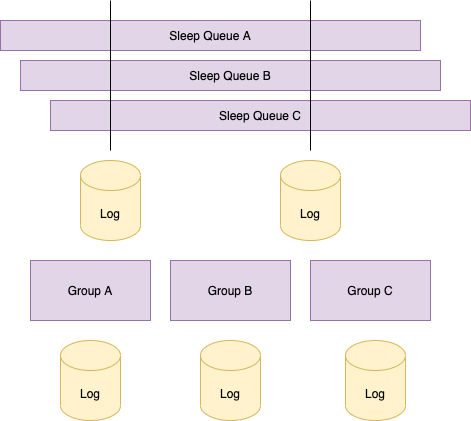
\includegraphics[width=\textwidth]{groupsleep.png}
\end{center}

\subsection{Sets and substitutions}

Ami can define a \textbf{set}, which could influence the value a field must have, by defining it explicitely, using the \textbf{field} keyword.
\begin{center}
field["fieldname"] = "value"
\end{center}

It is also possible to define a field to look for and assign a value to replace it with, such as:
\begin{center}
  field["ip"].replace("10.0.0.1" =$>$ "172.16.0.23", "10.2.3.4" =$>$ "172.16.0.254")
\end{center}

This is the syntax Pcraft will interpret as:
\begin{itemize}
  \item Search for the value "10.0.0.1" in the field "ip" and replace it with "172.16.0.23"
  \item Search for the value "10.2.3.4" in the field "ip" and replace it with "172.16.0.254"
\end{itemize}


\section{Pcraft Project}

Pcraft is built around the Ami language which defines the scenario and offers tools, such as "amidebug" to debug a given scenario and break step by step to read its content.

\begin{center}
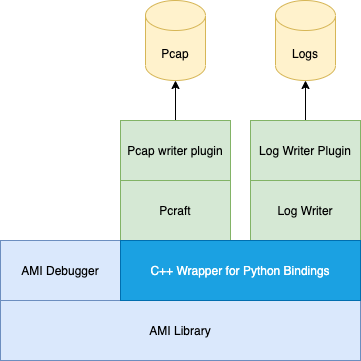
\includegraphics[width=10cm]{pcraft.png}
\end{center}

Pcraft is actually a C library which powers the Python one. Pcraft plugins are written in Python. Plugins offer the Packet Crafting capability, as well as the log template logic. This section will go into details on what those plugins can deliver.

\subsection{Pcraft plugins for Packet Writing}

Until now, by following this documentation you only wrote a DNS request and reply (\textbf{DNSConnection}) and used the \textbf{Void} plugin. Each plugin is called from using the \textbf{exec} keyword in an action.

\begin{lstlisting}[caption={Packet Writing plugins},captionpos=b]
  action useplugin {
    exec PluginName
  }
\end{lstlisting}

In the previous listing, \textbf{line 2}, the \textbf{PluginName} can be one of those: Controller, DNSConnection, FakeNames, HTTPConnection, PCAPImport, Ping, Suricata, TcpRst, TcpSynAck or Void.

\subsubsection{Controller}

The \textbf{Controller} plugin is used to create specific data that is not Network Data, such as Endpoint. It will not create a typical TCP/IP request and reply. To operate, this plugin must have the \textbf{\$log\_plugin} variable set. This variable will then call the proper log writer plugin.

Also, data created by this plugin must be encoded into fields sets.

\textbf{Example}

\begin{lstlisting}[caption={Controller plugin writing Windows User Login},captionpos=b]
  action user_logon {
    $log_plugin = "Controller"
    
    field["event_id"] = "4624"

    field["winlog_event_data_IpPort"] = random.int(10000, 60000)
    field["winlog_event_data_SubjectUserName"] = $username
    field["winlog_event_data_LogonGuid"] = uuid.v5($username)
    
    exec Controller
  }
\end{lstlisting}

\subsubsection{DNSConnection}

The \textbf{DNSConnection} plugin write a DNS request and reply. Those variables can be used: \textbf{\$ip-src}, \textbf{\$ip-dst}, \textbf{\$protocol}, \textbf{\$resolver}, \textbf{\$port-src}, \textbf{\$port-dst}, \textbf{\$domain}.

\subsubsection{FakeNames}

The \textbf{FakeNames} plugin creates a fake user and defines four variables: \textbf{\$firstname}, \textbf{\$lastname}, \textbf{\$name} and \textbf{\$domain}.

If the \textbf{\$orgdomain} variable is not defined, it will defaults to \textbf{yoda.com}.

\subsubsection{HTTPConnection}

The \textbf{HTTPConnection} plugin create an HTTP request and reply. The variables it can use as input are: \textbf{\$ip-src}, \textbf{\$ip-dst}, \textbf{\$protocol}, \textbf{\$domain}, \textbf{\$port-src}, \textbf{\$port-dst}, \textbf{\$ssl}, \textbf{\$method}, \textbf{\$user}, \textbf{\$user-agent}, \textbf{\$uri}, \textbf{\$resp-httpver}, \textbf{\$resp-code}, \textbf{\$resp-server}, \textbf{\$resp-content-type}, \textbf{\$resp-content}, \textbf{\$client-headers}, \textbf{\$client-content}.

\subsubsection{PcapImport}

This plugin will import a Pcap into the flow, and requires the \textbf{\$filename} variable to be set. Then with the field replacement, it can replace the IP addresses defined.

Also, it is possible to set the \textbf{\$onlyreplace} variable to \textbf{"true"} to force the import of only the IP addresses that are being replaced, discarding the other.

\textbf{Example}

\begin{lstlisting}[caption={Importing a Pcap file},captionpos=b]
  action pcapin {
    $filename = "myfile.pcap"
    $onlyreplace = "true"
    
    field["ip"].replace("10.0.0.1" => $client-ip)
    
    exec PcapImport
  }
\end{lstlisting}

\subsubsection{Ping}

Given an \textbf{\$ip-src} and \textbf{\$ip-dst}, it will generate an ICMP echo request and reply.

\subsubsection{Suricata}

Use a Suricata rule as input to create the wanted pcap that would trigger an alert. This feature works only on a subset of alerts and is highly experimental.

\textbf{Example}

\begin{lstlisting}[caption={Suricata crafting},captionpos=b]
action SuricataRule {
       exec Suricata
       $EXTERNAL_NET = "192.168.0.55"
       $HTTP_SERVERS = "141.193.213.20"
       $ip-dst = "141.193.213.20"
       $domain = "grayhat.co"
       $rule = """alert http $EXTERNAL_NET any -> $HTTP_SERVERS any (msg:"ET WEB_SERVER Possible Custom Content Type Manager WP Backdoor Access"; flow:established,to_server;http.uri; content:"/plugins/custom-content-type-manager/auto-update.php"; fast_pattern; nocase; reference:url,blog.sucuri.net/2016/03/when-wordpress-plugin-goes-bad.html; classtype:trojan-activity; sid:2022596; rev:4; metadata:created_at 2016_03_06, updated_at 2020_06_24;)"""
}
\end{lstlisting}

\subsubsection{TcpRst}

Create an exchange where \textbf{\$ip-src} sends a TCP packet with the SYN flag towards \textbf{\$ip-dst} and receives a TCP with the RST|ACK flags.

\subsubsection{TcpSynAck}

Create an exchange where \textbf{\$ip-src} sends a TCP packet with the SYN flag towards \textbf{\$ip-dst} and receives a TCP with the SYN|ACK flags. Then \textbf{\$ip-src} returns an ACK. This is a typical TCP/IP three way handshake.

\subsubsection{Void}

Debugging plugin, it will dump of the available variables at the time of its execution.


\section{Building Scenarios tips}

A typical scenario stores required information in a CSV, such as users, etc. and iterates through it to write the wanted event. It would use the group sleep feature to have one sleep pattern per user or machine one want data simulated from and the heavy use of loops help to fetch a given field to set the appropriate consistent value.

Do not forget to use the \textbf{delete} keyword to remove unwanted variables as soon as one does not need it.

The \textbf{message} function is a great way to debug thing you may want to understand on the fly, such as the \$index number or a variable content.

We can use the keyword \textbf{exit} at anytime, which would exit the parsing of the file when encoutered, allowing to debug the scenario.

The \textbf{skip\_repeat} keyword is also useful to run everyone once, thus avoiding getting into repeat loops for the sake of debugging.


\end{document}
